
\section{Chevron plot}

Now that we found an estimation of the interaction point, it's time to calibrate the gate~\cite{Gu2021}.

First we look back at \cref{fig:avoided_crossing} that was also showing the evolution of a state starting in $\ket{10}$.
Indeed if we prepare a state $\ket{10}$, using an already calibrated \pipulse on the first qubit, we can follow it up with a second pulse that moves the state along the orange curve.
This second pulse will be applied to qubit B and sent through the flux line on the qubit.
Ideally, there is no movement along the line, but only jumps: in the sense that, if we want to send a certain flux, we would like to not have any transient.
Because of this the flux pulse is initially defined as a rectangular pulse.

Let's try to understand the arrows drawn in \cref{fig:avoided_crossing}.
If we send a flux pulse with a flux of $0.1$ (considering the numbers in the plot) this will not be enough to reach the interaction point and, after the flux pulse in ended, measuring the two qubits will show that we still have a $\ket{10}$ state.
The same thing happen, more or less, if more flux than needed in sent.

If the flux value is correct, Rabi-like oscillations are produced between the two states as indicated in \cref{eq:iswap_oscillations}.
Actually, even at wrong fluxes we still achieve some Rabi-like oscillations, but with lower amplitude, higher frequencies, and lots of leakage to higher levels.

What we want to calibrate then, is the exact value of the flux needed for the two-qubit gate and the time $T$ to achieve the gate.
We perform an experiment with the following pulse sequence:
\begin{itemize}
    \item a first \pipulse is sent to qubit A (lower frequency);
    \item afterwards, a flux pulse in sent to qubit B (higher frequency);
    \item afterwards, a measurement is performed on both qubits;
    \item the experiment is repeated for various biases (around the expected crossing point) and various lengths.
\end{itemize}

The results of this experiment are plotted in a 3D graph with pulse-flux Vs pulse-length Vs $P_{01}$.
The z axis can actually represents different parameters: in particular probabilities regarding single qubit measurements (both for qubit A and B) or two-qubits measurement or, again, amplitude (defined as $\sqrt{i^2 + q^2}$) measurements.
Something that can happen, in particular for CZ where the second excited state is involved, is leakage outside the computing space that is usually not discriminated\footnote{A possibility it's then to discriminate also the state 2 (on top of 0 and 1) in the IQ plane.}.
Therefore it's usually preferred to use amplitude in case of CZs, while for iSWAP both probabilities and amplitude should work fine.

The expected plot for this experiment is presented in \cref{fig:chevron_sketch}.

\begin{figure}[htbp]
    \centering
    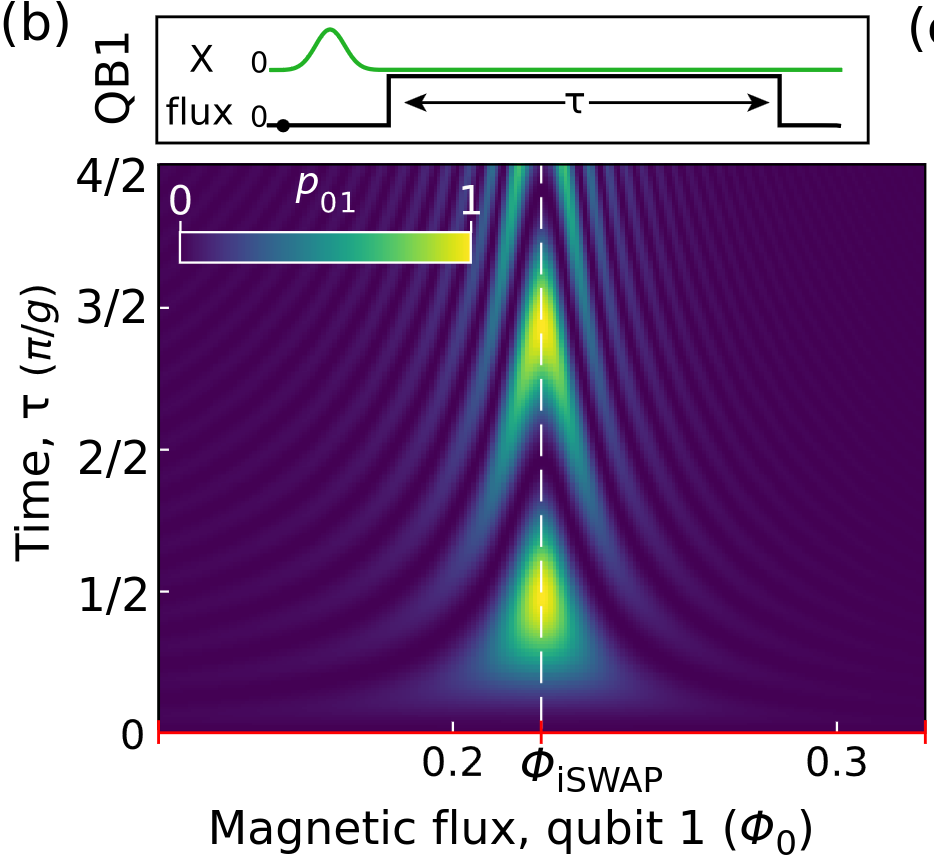
\includegraphics[width=8cm]{Two-qubits calibration/Figures/chevron_sketch.png}
    \caption{Expected plot for a two-qubits chevron.}
    \label{fig:chevron_sketch}
\end{figure}

This experiment, performed with the ZCU216 using the coded \Qibocal routines is presented in \cref{fig:nice_chevron}.

\begin{figure}[htbp]
    \centering
    \makebox[\textwidth][c]{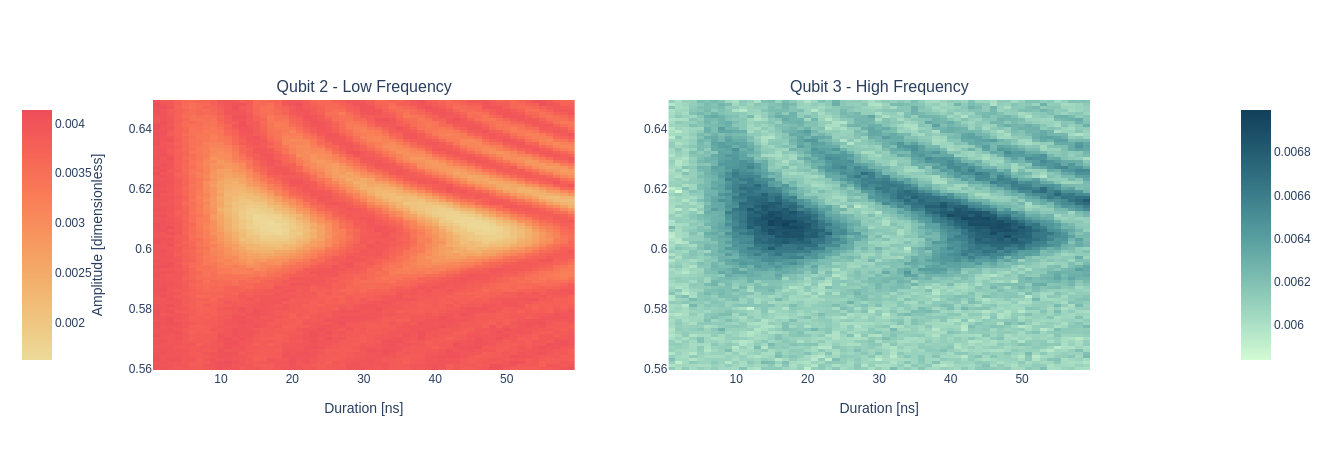
\includegraphics[width=1.3\textwidth]{Two-qubits calibration/Figures/good_chevron.png}}
    \caption{Chevron plot for CZ.}
    \label{fig:nice_chevron}
\end{figure}

The flux required for the two-qubits gate is the center one in the chevron plot, while the length of the pulse is chosen as half of the distance between two consecutive peaks at that flux (exactly as in the Rabi experiment).

